\documentclass[10pt]{article}
\usepackage{geometry}                
\geometry{a4paper}
\usepackage{graphicx}
\usepackage{amssymb}
\usepackage{amsmath}
\usepackage{paralist}
\usepackage[parfill]{parskip}
\usepackage{float}
\usepackage{capt-of}


\title{TMA4215 Numerical Mathematics: Project 2 \\ Replace this line with your own title} 
\author{Student nr. 6XXXXX and 7XXXXX} % Here you insert the student number of the members of the group.
\date{\today}

                                          
\begin{document}
\maketitle
\begin{abstract}

Bla bla Her kjem Abstract, men eg berre skriv litt for aa setje av plass til det. \\
Jepsi pepsi \\
Bezier er bra \\
Hurra \\

\end{abstract}

\section{Introduction} 

Bla bla Her kjem Introduction, men eg berre skriv litt for aa setje av plass til det. \\
Jepsi pepsi \\
Bezier er bra \\
Hurra \\
Tralalala \\
Eg er litt gal. \\

\section{Theory}



\subsection*{Bezier curves and Bernstein polynomials}

We have used Bezier curves to approximate a given curve $\gamma$. These are parametrized curves consisting of sums of Bernstein polynomials. A Bernstein polynomial is a polynomial of the form
\begin{align}
B_{i}^n(t) = \binom{n}{i}t^i(t-1)^{(n-i)},\quad i = 0, 1, ..., 0,\quad t \; \in \; [0,1],
\end{align}
and a bezier curve of degree n is given by
\begin{align}
\mathbf{S}(t) = \sum_{i=0}^{n} \mathbf{P_i} B_{i}^n(t), \quad 0 \leq t \leq 1,
\end{align}
where $\mathbf{P}_i$ are so called control. These points are chosen such that $\mathbf{P}_o$ and $\mathbf{P}_n$ are interpolation points between the Bezier curve and $\gamma$. In this report we are using cubic Bezier curves for solving the curve fitting problem, which means that each Bezier curves is made out of 4 points. $\mathbf{P}_0$ and $\mathbf{P}_3$ are end points, and $\mathbf{P}_1$ and $\mathbf{P}_2$ are points giving the curvature.



\subsection*{The least mean square problem}

For the best fit, $\mathbf{P}_1$ and $\mathbf{P}_2$ have to be chosen such that the distance between $\gamma$ and our bezier curve is the small. That is, we needed to minimize the the following expression:

\begin{equation}
E = \frac{1}{m} \sum_{i=1}^{m} \| \mathbf{x}_i - \mathbf{S}(t_i)\|^2_2,
\end{equation}

for parametrization values $t_i \in [ 0,1 ]$ and points $\mathbf{x}_i$ on $\gamma$. To do this we use a property of the Bezier curves: The two straight lines between $\mathbf{P}_0$ and $\mathbf{P}_1$, and $\mathbf{P}_2$ and $\mathbf{P}_3$ are tangents, $\mathbf{v}_0$ and $\mathbf{v}_3$, to the curve at $\mathbf{P}_0$ and $\mathbf{P}_3$ respectively:

\begin{align}
\mathbf{P}_1 = \mathbf{P}_2 + \alpha_1 \mathbf{v}_0 \\
\mathbf{P}_2 = \mathbf{P}_2 + \alpha_2 \mathbf{v}_3
\end{align}

Since $\mathbf{P}_0$ and $\mathbf{P}_3$ are known from the points on the curve $\gamma$, this problem is reduced to finding $\alpha_1$ and $\alpha_2$ such that $E$ is small. To find where $E$ is smallest, we differentiate $E$ with respect to $\alpha_1$ and $\alpha_2$ and set the expressions to equal zero. To ease the reader we omit the whole process, and only state the resulting system of equations for $\alpha_1$ and $\alpha_2$:


\begin{align}
\alpha_1 \sum_{i = 1}^m B_1(t_i)^2 |\mathbf{v}_0|^2 + \alpha_2 \sum_{i = 1}^m B_1(t_i)B_2(t_i)\mathbf{v}_0 \cdot \mathbf{v}_3 
= - \sum_{i = 0}^m B_1(t_i) \mathbf{v}_0 \cdot \mathbf{A}_i, \\
\alpha_1 \sum_{i = 1}^m B_1(t_i)B_2(t_i)\mathbf{v}_0 \cdot \mathbf{v}_3 + \alpha_2 \sum_{i = 1}^m B_2(t_i)^2 |\mathbf{v}_3|^2 
= - \sum_{i = 0}^m B_1(t_i)\mathbf{v}_3 \cdot \mathbf{A}_i,
\end{align}

where $\mathbf{A}_i = \mathbf{P}_0(B_0(t_i) + B_1(t_i) + \mathbf{P}_3(B_3(t_i) + B_2(t_i)) - \mathbf{x}_i$.





\subsection*{Choosing initial $t$-values and Newton-Raphson Iteration}

Choosing the initial $t$-values can be done in many ways. The easiest is probably to generate values ranging from 0 to 1 with equal distance, using the known command "linspace" in MATLAB. But is this really the parametrization that gives the smallest distance between the Bezier curve and $\gamma$? To see if it is we differentiate the distance between the two curves,
\begin{align}
(S_x(t) - x)^2 + (S_y(t) - y)^2,
\end{align}
with respect to $t$, where $S_x$ and $S_y$ are x- and y-coordinates on the Bezier curve, and $x$ and $y$ are coordinates on $\gamma$. We equate it to zero to find it's minimum, and we end up with a fifth-degree equation for $t$:
\begin{align}
f(t) =  2(X(t)-x)X'(t) + 2(Y(t)-y)Y'(t) = 0.
\end{align}
To find the solution we use the Newton-Raphson iterative method:
\begin{align}
t \gets t - \frac{f(t)}{f'(t)},
\end{align}
which will converge for the right starting values for $t$. We use initial $t$-values given by the distance between the data points, $x$ and $y$, from the curve $\gamma$. This method is merely based on \cite{Plass:1983}. Let

\begin{equation}
s_k = \sum_{i=1}^{k-1} \sqrt{(x_{i+1}-x_i)^2 + (y_{i+1}-y_i)^2}
\end{equation}

be the length of the polygonal segment from 1 to $k$, $k$ = 1, 2, ..., $n$. The initial parametric value is then $t_k = s_k/s_n$.

As seen from Figure \ref{fig:Newton-Raphson}, this method converges quickly, so few steps are required for a $t$-value close enough to the root. We can see how the $t$-values in Figure \ref{fig:Newton-Raphson} are quite shifted after 3 iterations, from the green lines to the red lines. It is important that the values are still in range 0 to 1, so this needs to be checked after the iterations. 




\begin{tabular}{ l c r }
  Initial & Iteration 3 & Iteration 7 & Iteration 8 \\ \hline
  0.0237 & 0.0165 & 0.0161 & 0.0161 \\ \hline
  0.1859 & 0.1429 & 0.1403 & 0.1403 \\ \hline
  0.2923 & 0.2439 & 0.2400 & 0.2399 \\ \hline
  0.4235 & 0.3969 & 0.3937 & 0.3937 \\ \hline
  0.5084 & 0.5115 & 0.5119 & 0.5120 \\ \hline
  0.6304 & 0.6701 & 0.6741 & 0.6742 \\ \hline
  0.7282 & 0.7770 & 0.7806 & 0.7807 \\ \hline
  0.8823 & 0.9136 & 0.9152 & 0.9153 \\ \hline
\end{tabular}


\begin{figure}[H]
    \centering
    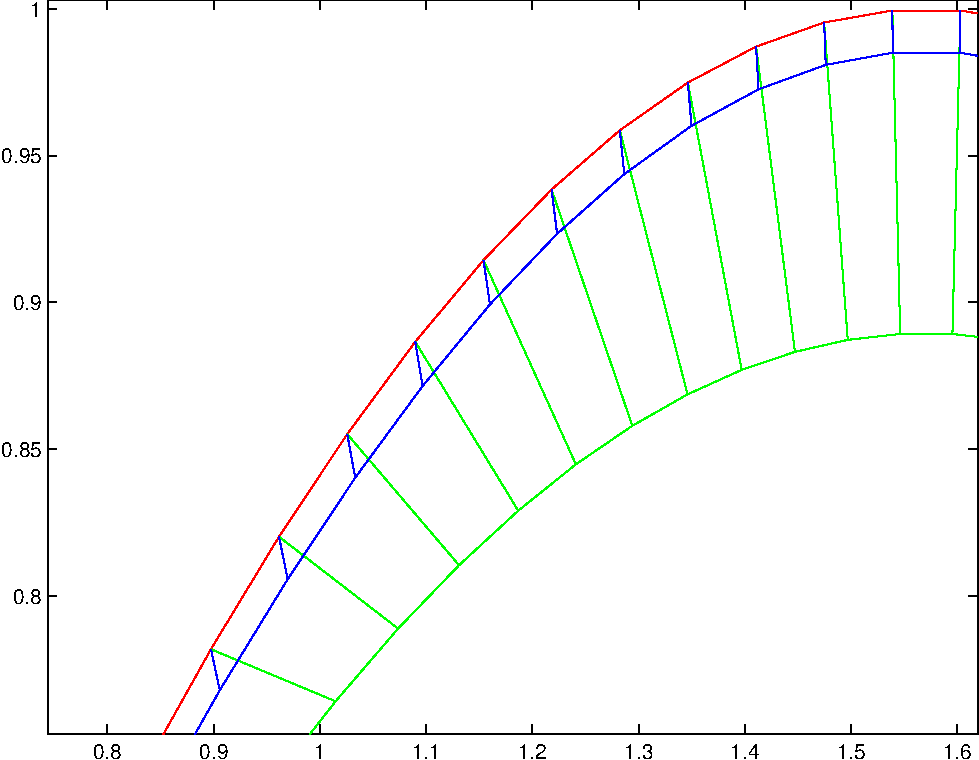
\includegraphics[scale=0.6]{newtons2-crop.pdf}
    \caption{Result after 3 Newton-Raphson iterations. The blue curve ($\gamma$) is a part of a sine function. The green curve is the Bezier curve with initial $t$-values. The red curve is the Bezier curve after 3 iterations. A straight line represents the distance between a point on $\gamma$ and the corresponding point on the Bezier curve.}
    \label{fig:Newton-Raphson}
\end{figure} 

With the new $t$-values, we can check the error between the Bezier curve and $\gamma$. If the error is still too big, it is possible to split the interval in two, and do new approximations for the $t$-values.



\subsection*{Unit tangent vectors}
To find the unit tangent vectors $\mathbf{v}_0$ and $\mathbf{v}_3$, we use the known data points $x$ and $y$ around the end points $\mathbf{P}_0$ and $\mathbf{P}_3$. We differ between tangent vectors from corners and tangent vectors that make the curve $C^1$.

A tangent vector that has its origin in a corner will only need data points from one side of the end point. That is, the slope of the vector $\mathbf{v}_i$ is measured by $m_i = (y_{i+r} - y_0)/(x_{i+r} - x_0)$, $r$ being a positive integer denoting the number of data points away from the end point. One way of choosing $r$ is defining it as a fraction of the total number of data points, rounded upwards to the closest integer (------------may use math notation here).
 The unit tangent vector is  $\mathbf{v}_i = \frac{[1, m_i]^T}{\sqrt{1+m_i^2}}$, where we have divided with the norm. If the denominator in $m_i$ is close to zero, the unit tangent vector might be badly scaled. To avoid this, we recommend $\mathbf{v}_i = [0,1]$ when $x_{i+r} - x_i$ is below some limit close to zero. 

If the error between a Bezier curve and the original curve is too large, the curve is divided in two, where the dividing point, hereby called $\mathbf{P}_i$ becomes new end points, $\mathbf{P}_0$ and $\mathbf{P}_3$, for the two Bezier curves. To obtain a curve that is $C^1$, the vector must be the tangent in $\mathbf{P}_i$ on the curve, with slope $m_i = (y_{i+r} - y_{i-r})/(x_{i+r} - x_{i-r})$. The unit tangent vector is computed in the same way as described earlier, such that $\mathbf{v}_i = \mathbf{v}_0 = -\mathbf{v}_3$. $\mathbf{v}_3$ is negative because it's pointing in the opposite direction. Remark that $i+r$ or $i-r$ sometimes might range outside the domain of the data points. 

If the shape to be fitted has smooth corners, one option is to make all end points $C^1$. This can be done by constructing one tangent vector in an optional point on the curve, and construct new tangent vectors in points from dividing the curve recursively.


\subsection*{Avoiding singular matrices}
When solving the system of equations above, a problem of a singular matrix may arise. We get a singular matrix when the tangent vectors, $\mathbf{v}_0$ and $\mathbf{v}_3$, are parallel, and this happens when the number of points in our subset of points are smaller than 3. This is because the previous described method of choosing tangent vectors will make them parallel if there are no points between them. To avoid this problem we include a space limitation in our algorithm. If the number of elements in a subset of points is smaller then a certain space parameter, we will not divide the curve any further.


\subsection*{Dividing the curve in two}
After using Newton-Raphson, if the error between $\gamma$ and the Bezier curve is still above the tolerance, it is possible to divide the curve in two. This can be done simply by choosing the point, $\mathbf{P}_i$, where the error is largest. If $\mathbf{P}_i$ is closer to one of the endpoints than a certain space parameter, we choose to split the curve, $\gamma$, in the midpoint. After splitting, we construct a Bezier curve for each half, using the same method recursively. 

If $\gamma$ has less than 3 points, splitting the curve will not make a better parametrization, since the tangent vectors in both end points will be the same, only with opposite directions.



Divide curve in two, recursive, largest distance
Singular matrices
divergent t-values


Tangent vectors
Corners, control points
Number of Bezier curves (Numerical section?
Figures are good!


\section{Numerical experiments}

In this section we will present the results of our algorithm run on different test problems. We will see how smoothness in the corners affects the imaging, and we will see the effects of different values for the space parameter and the error tolerance.






\section{Conclusion}
\cite{Plass:1983}

\bibliographystyle{plain}
\bibliography{bezierbib}   % Insert you own BibTeX file 
\end{document}  
